\chapter{背景}
\label{background}
\section{ボディビルディングについて}

競技ボディビルは、選手が日頃の厳しいトレーニングにより鍛え上げた筋肉の発達度や美しさ、バランスを競う個人スポーツである。競技方法として、エントリーした選手の中から予選審査(プレジャッジ)を経て10~12名が選ばれ、これらの選手による比較審査が行われる。
選手は司会者の指示に従い、規定のポーズを取り、音楽に合わせたフリーポーズも披露する。予選審査では上位に進む選手を選出し、後半で上位選手同士が厳密に評価される。
決勝審査では、プレジャッジで選ばれた上位選手がフリーポーズを披露し、審査員による合計点で順位が決まる。\cite{bodybuilding}審査基準は筋肉の大きさ、形、明瞭さ、バランス、ポーズの流れ、表現法などである。

規定ポーズは、コンパルソリー(compulsory)ポーズと呼ばれ、同じポーズで
比較すると云う意味になる。同時に決まったポーズをとることは、選手すべてが同じ型
のポーズで同じ条件のもとに比較されると云うことになる。\cite{posing_performance_jbbf} \\
男子ボディビルでは
\begin{enumerate}
    \item フロント ダブルバイセプス 図\ref{fig:double_biceps}
    \item フロント ラットスプレッド 図\ref{fig:front_lat_spread}
    \item サイド チェスト(エニーサイド) 図\ref{fig:side_chest}
    \item バック ダブルバイセプス 図\ref{fig:back_double_biceps}
    \item バック ラットスプレッド 図\ref{fig:back_lat_spread}
    \item サイド トライセプス(エニーサイド) 図\ref{fig:side_triceps}
    \item アブドミナル アンド サイ 図\ref{fig:abdominal_and_sai}
\end{enumerate}

\begin{figure}[H]
    \centering
    \begin{tabular}{ccc}
        \begin{minipage}[t]{.33\textwidth}
            \centering
            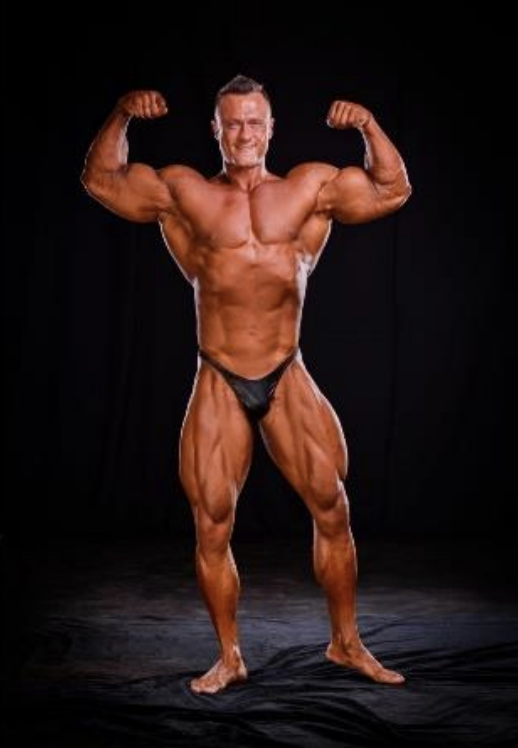
\includegraphics[width=0.75\linewidth, height=5cm]{figures/double_biceps.png}
            \caption{フロントダブルバイセップス}
            \label{fig:double_biceps}
        \end{minipage} &
        \begin{minipage}[t]{.33\textwidth}
            \centering
            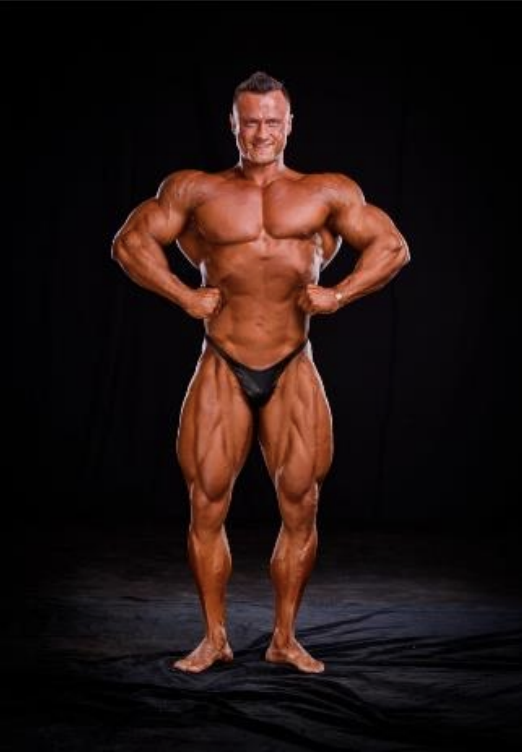
\includegraphics[width=0.75\linewidth, height=5cm]{figures/front_lat_spread.png}
            \caption{フロントラットスプレッド}
            \label{fig:front_lat_spread}
        \end{minipage} &
        \begin{minipage}[t]{.33\textwidth}
            \centering
            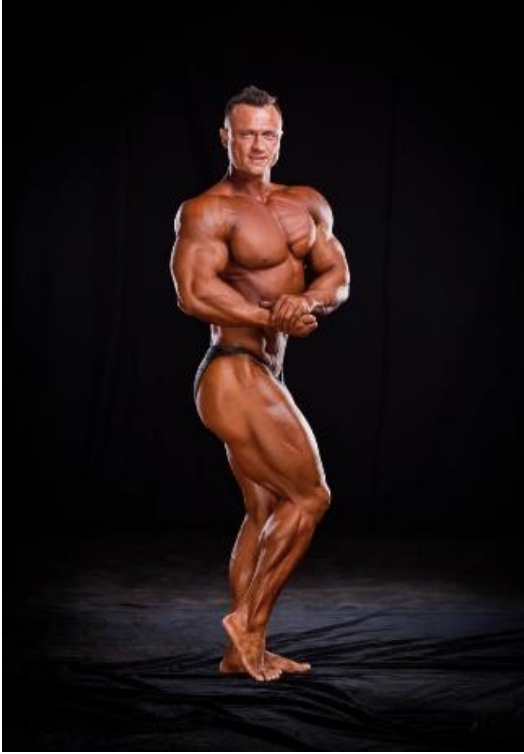
\includegraphics[width=0.75\linewidth, height=5cm]{figures/side_chest.png}
            \caption:サイドチェスト
            \label{fig:side_chest}
        \end{minipage}
    \end{tabular}

    \begin{tabular}{cccc}
        \begin{minipage}{.25\textwidth}
            \centering
            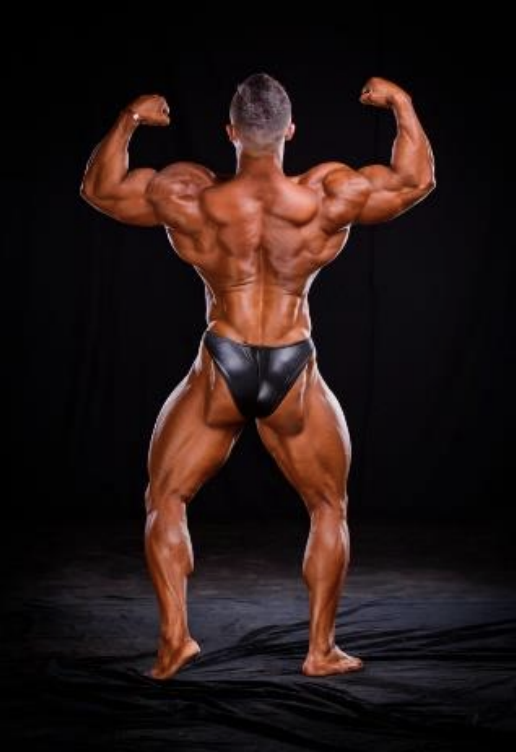
\includegraphics[width=0.75\linewidth, height=3.75cm]{figures/back_double_biceps.png}
            \caption{バックダブルバイセップス}
            \label{fig:back_double_biceps}
        \end{minipage} &
        \begin{minipage}{.25\textwidth}
            \centering
            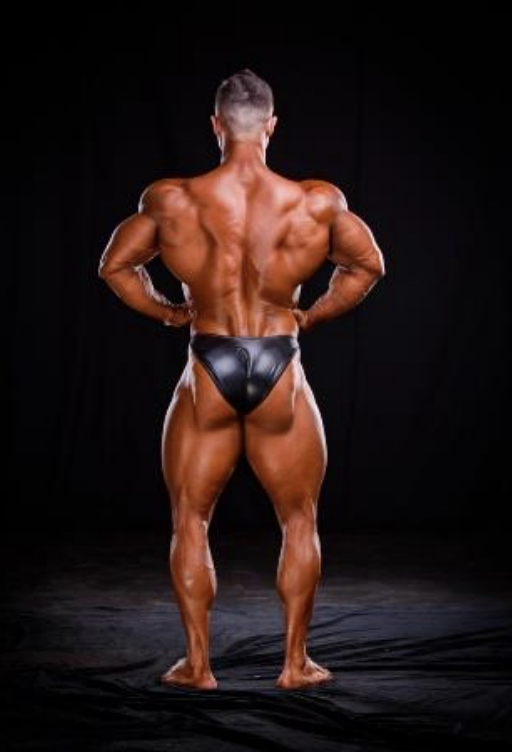
\includegraphics[width=0.75\linewidth, height=3.75cm]{figures/back_lat_spread.png}
            \caption{バックラットスプレッド}
            \label{fig:back_lat_spread}
        \end{minipage} &
        \begin{minipage}{.25\textwidth}
            \centering
            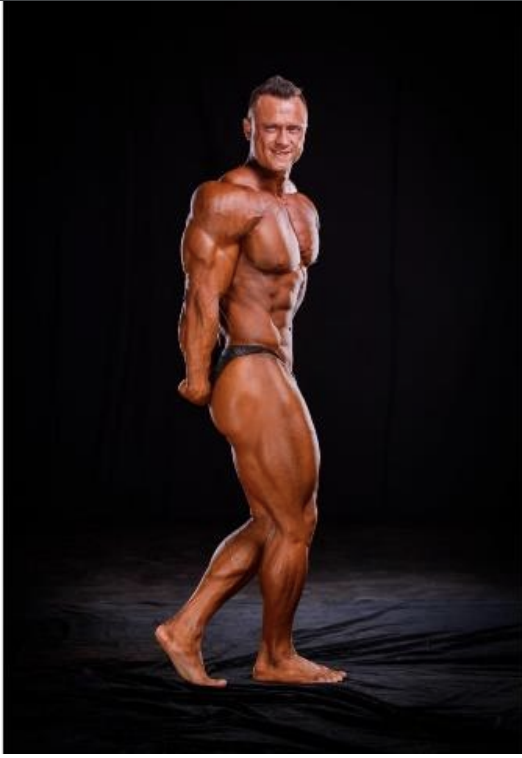
\includegraphics[width=0.75\linewidth, height=3.75cm]{figures/side_triceps.png}
            \caption{サイドトライセップス}
            \label{fig:side_triceps}
        \end{minipage} &
        \begin{minipage}{.25\textwidth}
            \centering
            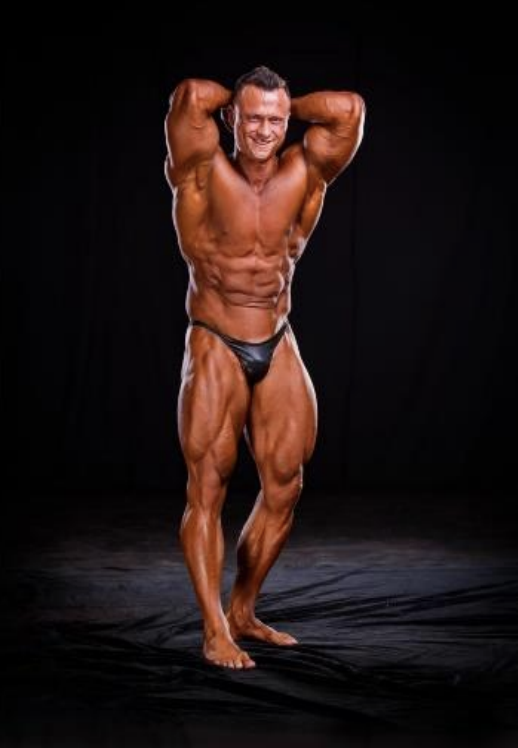
\includegraphics[width=0.75\linewidth, height=3.75cm]{figures/abdominal_and_sai.png}
            \caption{アブドミナルアンドサイ}
            \label{fig:abdominal_and_sai}
        \end{minipage}
    \end{tabular}
\end{figure}



の7ポーズが規定ポーズである。この規定ポーズと前後左右のリラックスポーズで比較される。

ポージングはボディビルにおいて大会当日にできる唯一の要素であり、鍛え上げてきた肉体をより良く見せるための重要なものである。
\section{骨格推定}
骨格推定とは深層学習などを用いて人物のポーズを可視化してくれる手法であり、モーションキャプチャーなどの機器を使用することなく,
画像、動画データ、又はカメラからの入力を用いて人間のポーズを可視化することができる。
カーネギーメロン大学(CMU)の Zhe Caoら が「Realtime Multi-Person pose estimation」\cite{openpose}の論文で発表した、OpenPoseが一つの例である。

\section{内在的フィードバック}
内在的フィードバックとは、私たちが動作を実行する際に自分の感覚に基づいてその動作を評価し、学習するプロセスである。例えば、歩行時に足の裏から伝わる路面の感覚を認識することや、自分の進む方向を視覚的に確認することも、この内在的フィードバックの一例であることと言える。\cite{nagoyahml_feedback}
\section{ガイダンス仮説}
ガイダンス仮説\cite{guidance_hypothesis}とは、フィードバックは学習者を正しい運動に導くガイドとなるが、もしフィードバックを頻繁に与えすぎた場合は、それに過度に依存して、内在的フィードバックの処理を無視するようになり、逆に悪影響を与えるという考えである。すなわち、外在的フィードバックを頻繁に与え過ぎることで学習者はそれに依存してしまい、内在的フィードバックの1つである運動感覚を利用した能動的な動作の修正を行わなくなる。
その結果、外在的フィードバックを伴う練習中においてはパフォーマンスが優れているものの、外在的フィードバックがない保持テストでは正確な運動を行えないことが多い。
\section{関連研究}
武蔵野大学の鎌田らは \cite{Relatedresearch1}スクワットのフォームに対してOpenPoseを用いて姿勢差分に用いる関節角度の抽出方法とについて実装した。
また、広島市立大学の岡本らは \cite{Relatedresearch2}陸上のハードル跨ぎの練習においてKinectを用いて骨格を推定し、リアルタイムでフィードバックを返すシステムを提案した。